%
% CMPT 379: Principles of Compiler Design - A Course Overview
% Section: Register Allocation
%
% Author: Jeffrey Leung
%

\section{Register Allocation}
	\label{sec:register-allocation}
\begin{easylist}

& Intermediate representation uses unlimited temporary storage locations, which must be translated to a limited number of registers
& \textbf{Live:} Variable which has been defined and is being used or will be used later
	&& Should be loaded into a register for quicker access
& \textbf{Liveness analysis:} Detection of when variables are and are not live
	&& Variables can share a register if, at all points in the program, no more than one of them are live
	&& At the end of each line of code, create a set of all live variables
	&& \textbf{Live range:} Locations in the program where a variable is live
	&& \textbf{Live interval:} Start and end line numbers which represent from when a variable is first defined to its last usage
		&&& Greedy algorithm can be applied to allocate registers based on when the live interval for a variable ends

& \textbf{Register Interference Graph (RIG):} Undirected graph where each node represents a unique temporary variable, and an edge $(t_1, t_2)$ exists iff they are both live at any given point in the program
	&& For two variables $v_1, v_2$, if there is no edge connecting them, they can be allocated to the same register
	&& E.g. For the RIG in figure~\ref{fig:example-register-interference-graph}, $a, c$ cannot be in the same register, but $a, d$ can be in the same register

\begin{figure}[!htb]
	\caption{Example of a Register Interference Graph}
	\label{fig:example-register-interference-graph}
	\begin{center}
		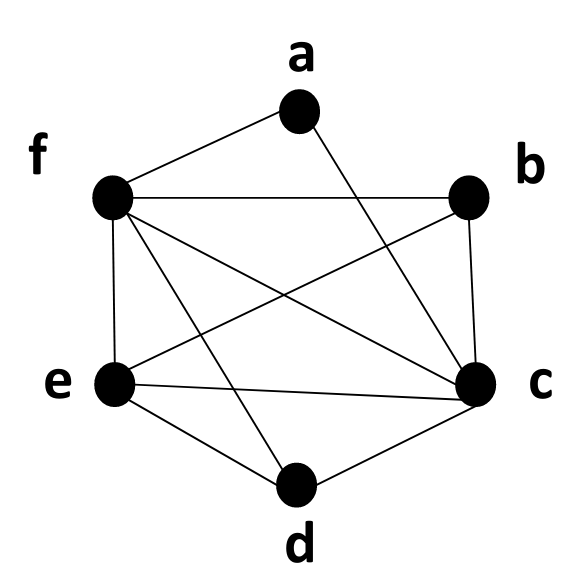
\includegraphics[width=0.4\textwidth]{register-interference-graph.png}
	\end{center}
\end{figure}

& \textbf{Spilling:} Operation which allocates a memory location for a variable when there are not enough registers to store all live variables
	&& When a variable must be spilled, the live range of the variable is reduced and the RIG is updated

& $k$-coloring problem: Given a graph, can $k$ colors be applied to the nodes such that each node has only one color, and no connected nodes share the same color?
	&& Apply the $k$-coloring problem to find the minimum possible coloring for the graph, where $k$ also equals the minimum number of registers required
	&& If $k$ is not large enough, then a node is spilled
	&& \textit{Optimistic coloring heuristic algorithm:}
		&&& Choose an arbitrary $k$ to attempt
		&&& Remove a node with less than $k$ neighbors and push it into a stack (repeat until the graph is empty)
		&&& Pop a node and connect it to its neighbors in the graph, then assign either an existing color or a new color (repeat until the stack is empty)

& \textbf{Linear scan register alllocation:} Algorithm which detects when a variable needs to be spilled
	&& Efficient
	&& Less effective than graph coloring

\end{easylist}
\clearpage
